%%
%% Appendix F: Additional figures
%% Figure admission rule: ONLY assets dispositioned INCLUDED-V / REGENERATED-V
%% by the Wave-0 provenance pass (thesis/PROVENANCE.md Sections 3/3a) and not
%% already consumed by Chapters 5-6. Every caption names its verification
%% basis, matching the corresponding PROVENANCE.md Class-V note.
%%
\chapter{Additional Figures}
\label{app:f}

This appendix collects qualitative figures that support the analyses of
Chapters~\ref{ch:05} and~\ref{ch:06} but did not fit the main text: skeleton
overlay examples from the pose-extraction stage
(Section~\ref{sec:appf-overlays}), additional temporal score curves beyond the
one shown in Chapter~\ref{ch:05} (Section~\ref{sec:appf-temporal}), the
gate-activation histograms complementing the per-category gate statistics of
Chapter~\ref{ch:05} (Section~\ref{sec:appf-gates}), and per-category
frame-score distributions (Section~\ref{sec:appf-catscores}). Every figure in
this appendix is registered in the thesis provenance manifest
(\texttt{thesis/PROVENANCE.md}) with a verification note recording what it was
checked against; the captions below summarize those notes. The Pri-9 score
histogram that an early draft assigned to this appendix appears in
Chapter~\ref{ch:05} instead and is not duplicated here. A number of
earlier exploratory charts (single-seed ablation and seed-stability bar
charts, and a cross-dataset comparison chart) were deliberately omitted from
this thesis because they embed superseded single-seed values already covered
--- at three-seed precision --- by the tables of Chapter~\ref{ch:05}.

\section{Skeleton Overlay Examples}
\label{sec:appf-overlays}

Figure~\ref{fig:appf-skel-overlays} shows RTMPose keypoint overlays on
XD-Violence source frames from the pose-extraction stage of
Chapter~\ref{ch:03}: two frames from a B1 (fighting) clip and one from a B2
clip, with the 17 COCO keypoints of the top-2 detected persons drawn over the
frame. The examples illustrate both what the skeleton stream sees --- clean
multi-person pose structure during close-quarters action --- and its known
failure surface: partially occluded limbs receive low-confidence keypoints,
which the confidence channel of the skeleton tensor exposes to the downstream
encoder.

These overlays are XD-Violence-only \emph{by necessity}, not by choice:
UCF-Crime is distributed as frames pre-sampled to $64\times64$ pixels
(Appendix~\ref{app:d}), a resolution at which rendered keypoint overlays are
not legibly interpretable --- the skeleton occupies a handful of pixels. Pose
extraction itself runs on UCF-Crime at that resolution (the pose model
operates on the detected person crop), but qualitative overlay figures are
only meaningful on XD-Violence's full-resolution frames.

% Source: thesis/PROVENANCE.md §3 rows fig_skeleton_overlay_b01/02/03 —
% Class V, byte-identical copies (cmp exit 0) of the phase-6 B-series
% renderings; overlays are independent of eval scores/checkpoints.
\begin{figure}[htbp]
  \centering
  \begin{subfigure}[t]{0.32\textwidth}
    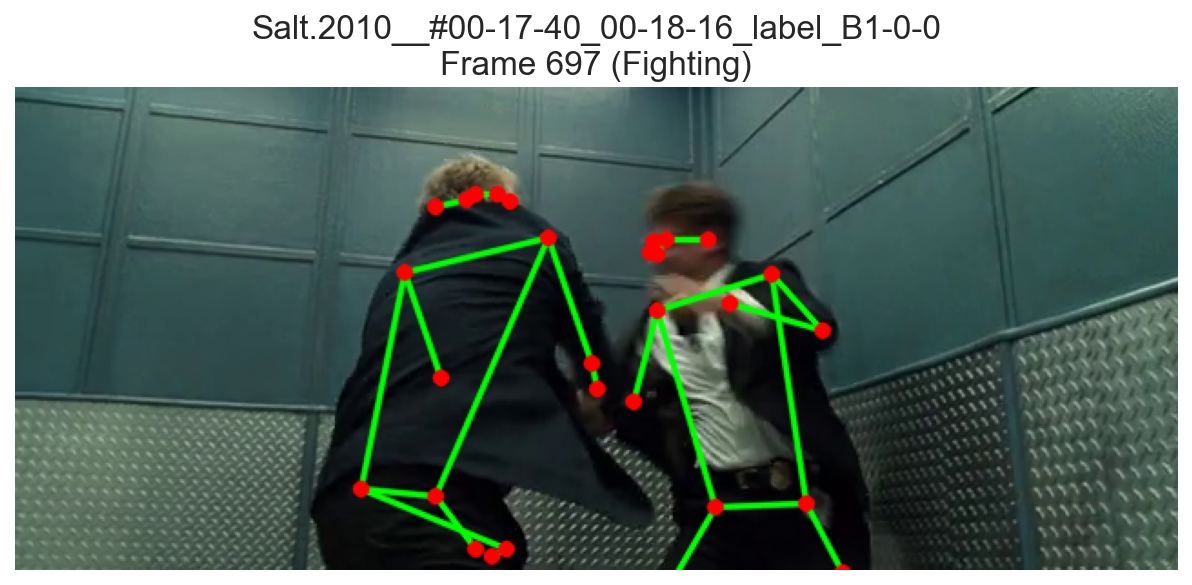
\includegraphics[width=\textwidth]{figures/fig_skeleton_overlay_b01}
    \caption{B1 clip (\emph{Salt}, 2010), frame 697.}
  \end{subfigure}\hfill
  \begin{subfigure}[t]{0.32\textwidth}
    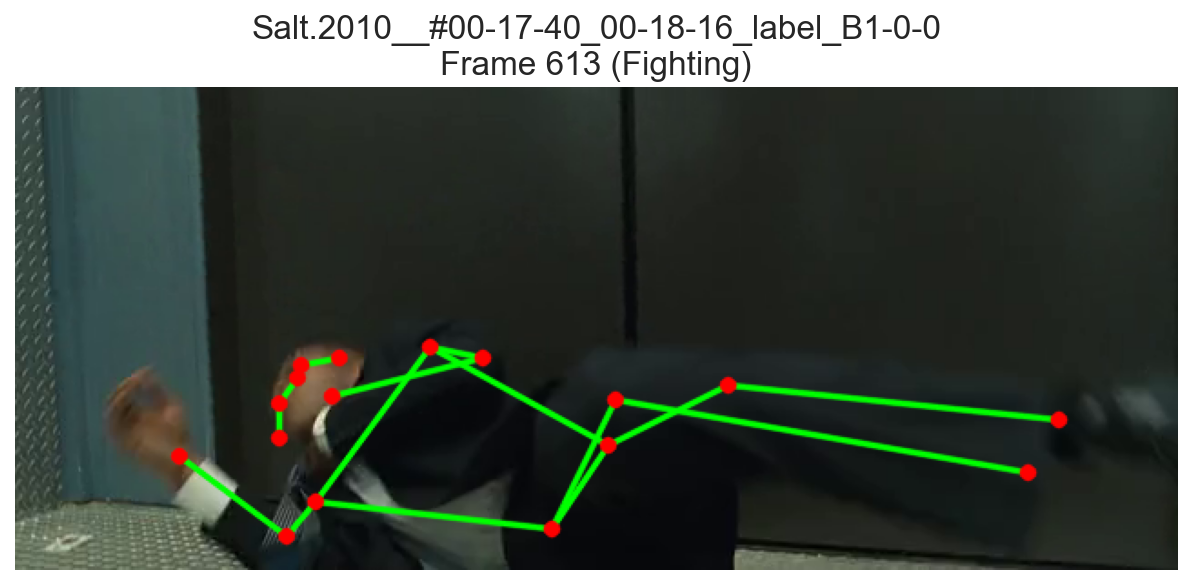
\includegraphics[width=\textwidth]{figures/fig_skeleton_overlay_b03}
    \caption{Same B1 clip, frame 613.}
  \end{subfigure}\hfill
  \begin{subfigure}[t]{0.32\textwidth}
    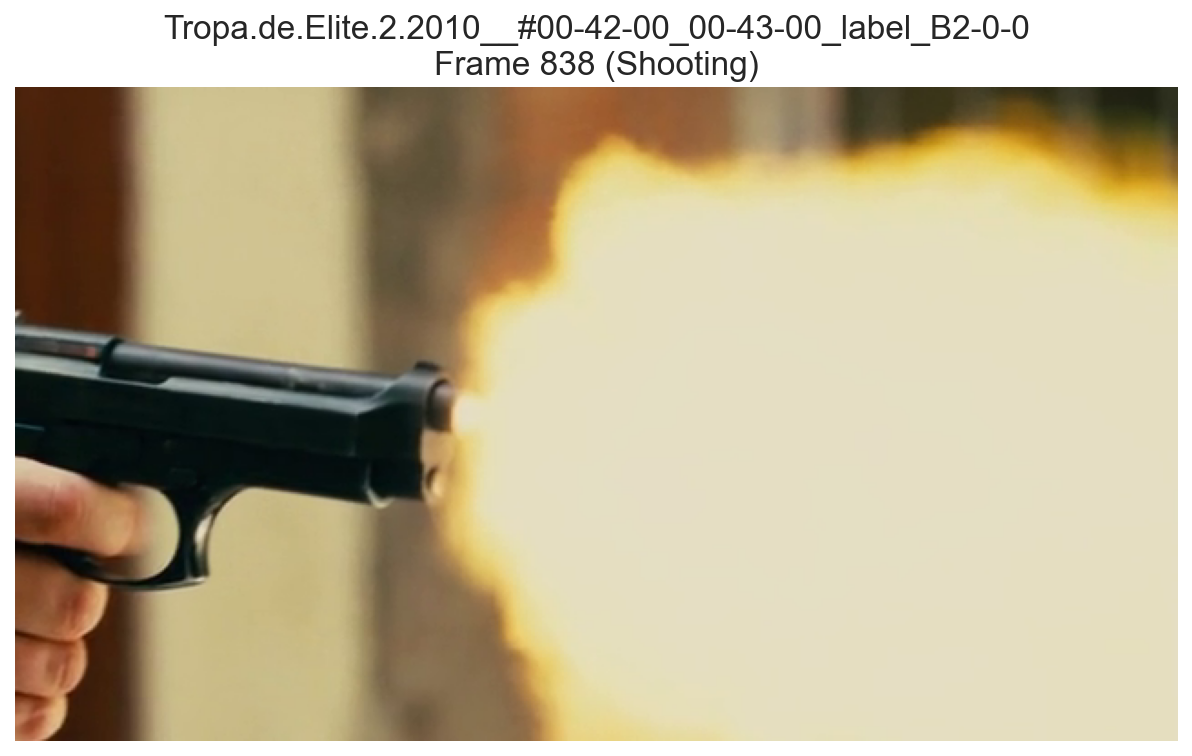
\includegraphics[width=\textwidth]{figures/fig_skeleton_overlay_b02}
    \caption{B2 clip (\emph{Tropa de Elite~2}), frame 838.}
  \end{subfigure}
  \caption{RTMPose keypoint overlays (17 COCO keypoints, top-2 persons) on
  XD-Violence source frames. Verification: byte-identical copies of the
  extraction-stage renderings; skeleton overlays depend only on the frozen
  pose extractor, not on any trained model or evaluation output, so no
  later pipeline change can stale them (PROVENANCE.md Class-V notes).
  UCF-Crime counterparts are omitted because its distributed frames are
  $64\times64$ pixels --- too small for legible overlays.}
  \label{fig:appf-skel-overlays}
\end{figure}

\section{Additional Temporal Score Curves}
\label{sec:appf-temporal}

Chapter~\ref{ch:05} shows one temporal score curve; Figures
\ref{fig:appf-temporal-ucf} and~\ref{fig:appf-temporal-xd} add three more
(two UCF-Crime, one XD-Violence), each comparing the four fusion variants'
frame-level anomaly scores over a full test video against the ground-truth
anomaly window. The UCF-Crime examples (Shooting008, Explosion033) show the
gated model localizing the annotated event where the skeleton-only score is
comparatively flat --- consistent with the visually-driven nature of those
categories --- while the XD-Violence example (\emph{Black Hawk Down}, a G
clip) shows sustained elevated scores across an extended action sequence.

% Source: thesis/PROVENANCE.md §3 rows fig_temporal_extra_* — Class V,
% regenerated 2026-07-05 from s42 score dumps validated EXACTLY (recomputed
% frame-level AUC/AP vs tracked eval_metrics.json, diff 0.00e+00, all runs).
\begin{figure}[htbp]
  \centering
  \begin{subfigure}[t]{\textwidth}
    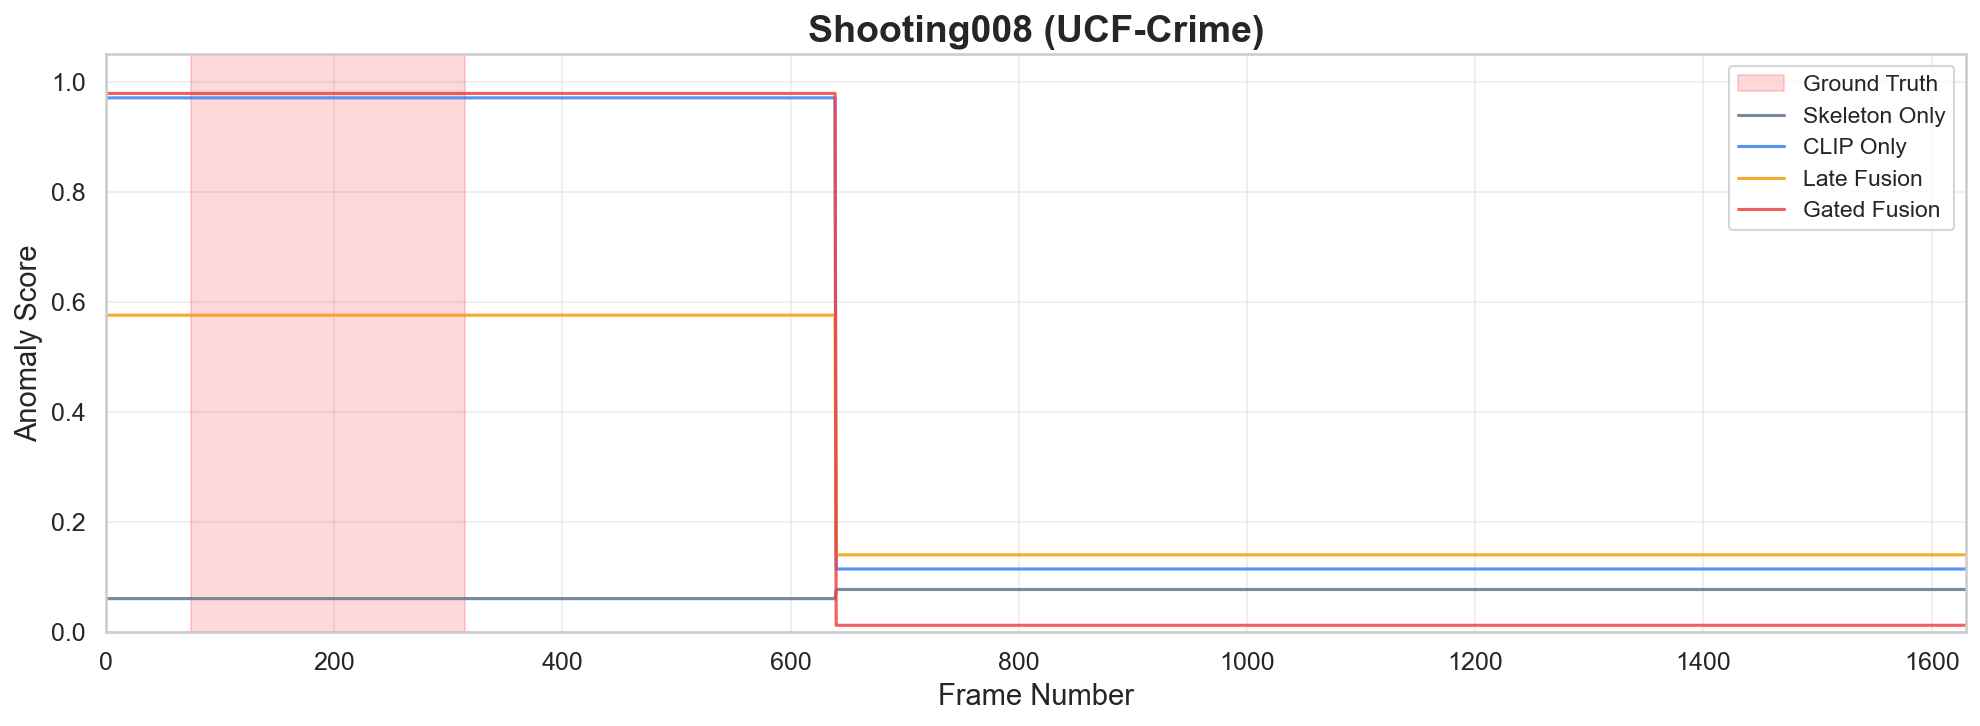
\includegraphics[width=\textwidth]{figures/fig_temporal_extra_ucf_shooting008}
    \caption{UCF-Crime, Shooting008.}
  \end{subfigure}\par\medskip
  \begin{subfigure}[t]{\textwidth}
    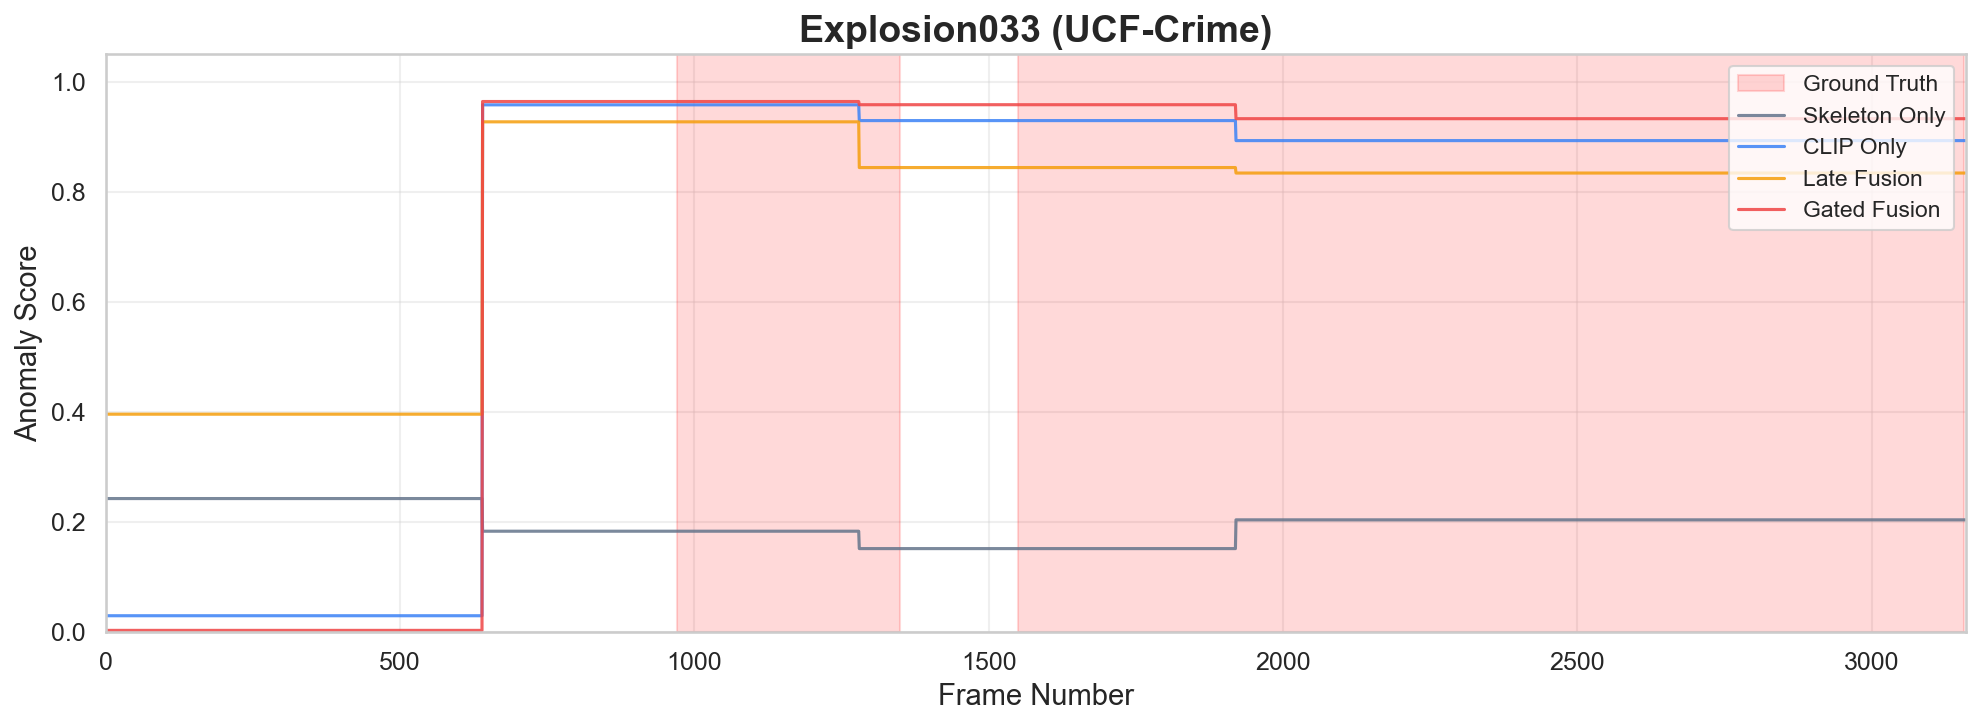
\includegraphics[width=\textwidth]{figures/fig_temporal_extra_ucf_explosion033}
    \caption{UCF-Crime, Explosion033.}
  \end{subfigure}
  \caption{Additional UCF-Crime temporal score curves (seed 42 models;
  shaded region marks the annotated anomaly window). Verification: curves
  regenerated from score dumps that were first validated against the tracked
  canonical metrics --- frame-level AUC/AP recomputed from each dump matches
  the tracked \texttt{eval\_metrics.json} exactly (PROVENANCE.md Class-V
  notes).}
  \label{fig:appf-temporal-ucf}
\end{figure}

\begin{figure}[htbp]
  \centering
  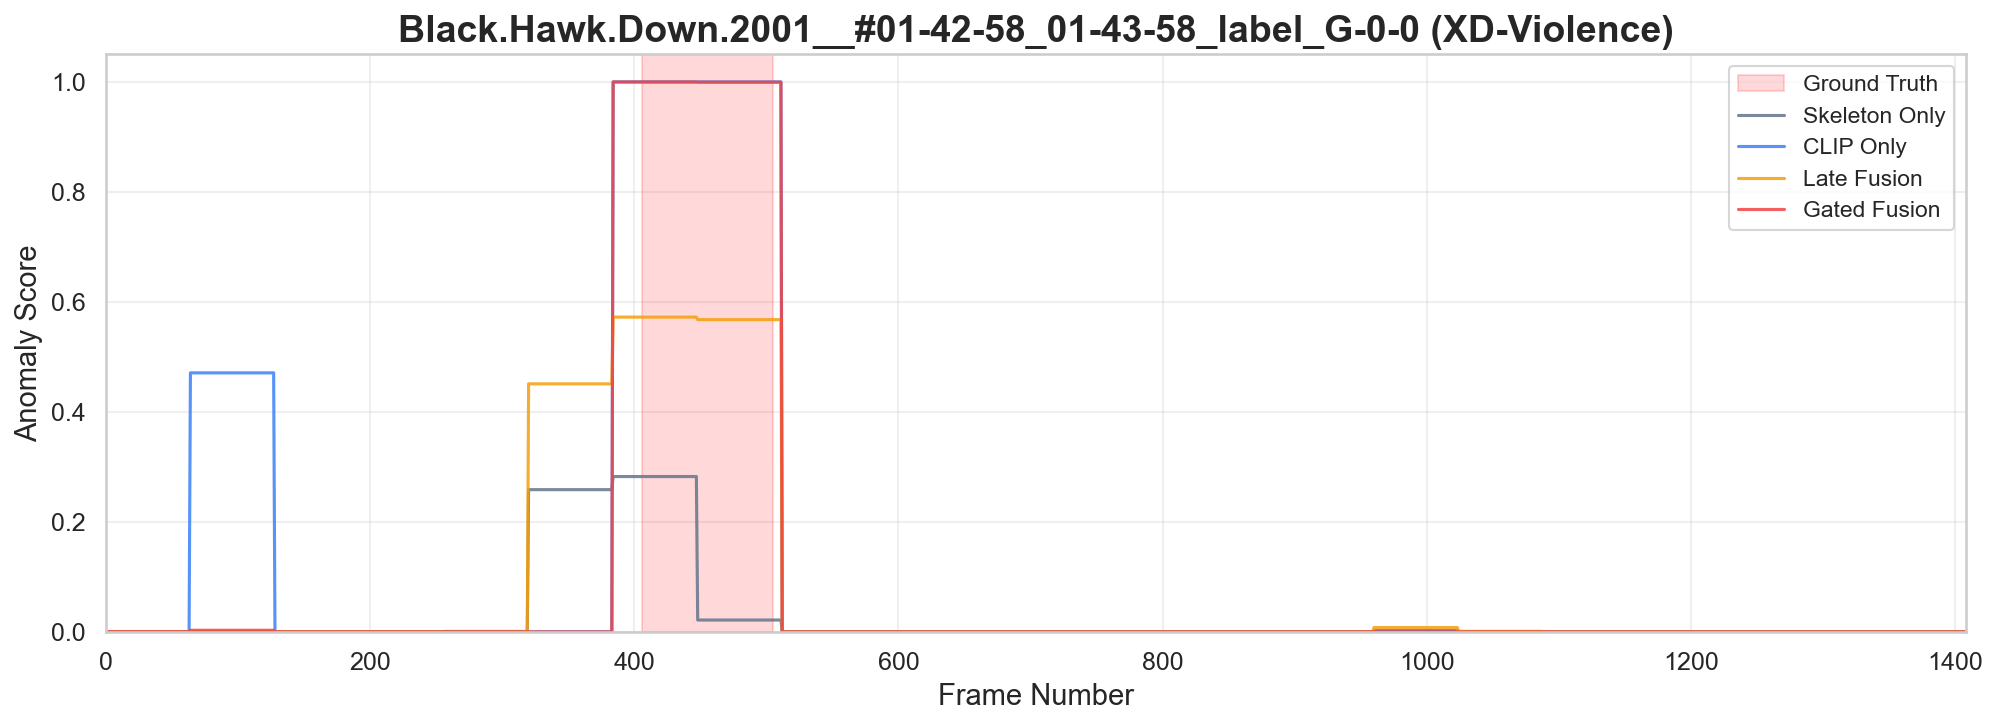
\includegraphics[width=\textwidth]{figures/fig_temporal_extra_xd_blackhawkdown}
  \caption{XD-Violence temporal score curve (\emph{Black Hawk Down}, G clip;
  seed 42 models; shaded regions mark annotated anomaly windows). Same
  verification basis as Figure~\ref{fig:appf-temporal-ucf}: the underlying
  score dump reproduces the tracked canonical metrics exactly before
  replotting (PROVENANCE.md Class-V note).}
  \label{fig:appf-temporal-xd}
\end{figure}

\section{Gate-Activation Histograms}
\label{sec:appf-gates}

Chapter~\ref{ch:05} reports per-category mean gate activations;
Figure~\ref{fig:appf-gate-hist} shows the full distribution of gate values,
separated into normal and anomalous test videos, for the gated-fusion models
on both datasets. Two properties are visible. First, the gate spans nearly
its entire $(0,1)$ range on both datasets rather than saturating --- the
learned weighting is genuinely input-dependent, not a fixed mixing constant
in disguise. Second, the normal and anomalous distributions overlap
substantially: the gate is not itself an anomaly detector, but a
modality-trust signal that varies with scene content within both classes.

% Source: thesis/PROVENANCE.md §3 rows fig_gate_histogram_{ucf,xd} — Class V,
% regenerated 2026-07-05 from the s42 gated-fusion checkpoints, each first
% verified: official src/evaluate.py CLI reproduces the tracked canonical
% auc/ap exactly (diff 0.00e+00). Includes the 13-04 UCF Normal-classification
% fix.
\begin{figure}[htbp]
  \centering
  \begin{subfigure}[t]{0.48\textwidth}
    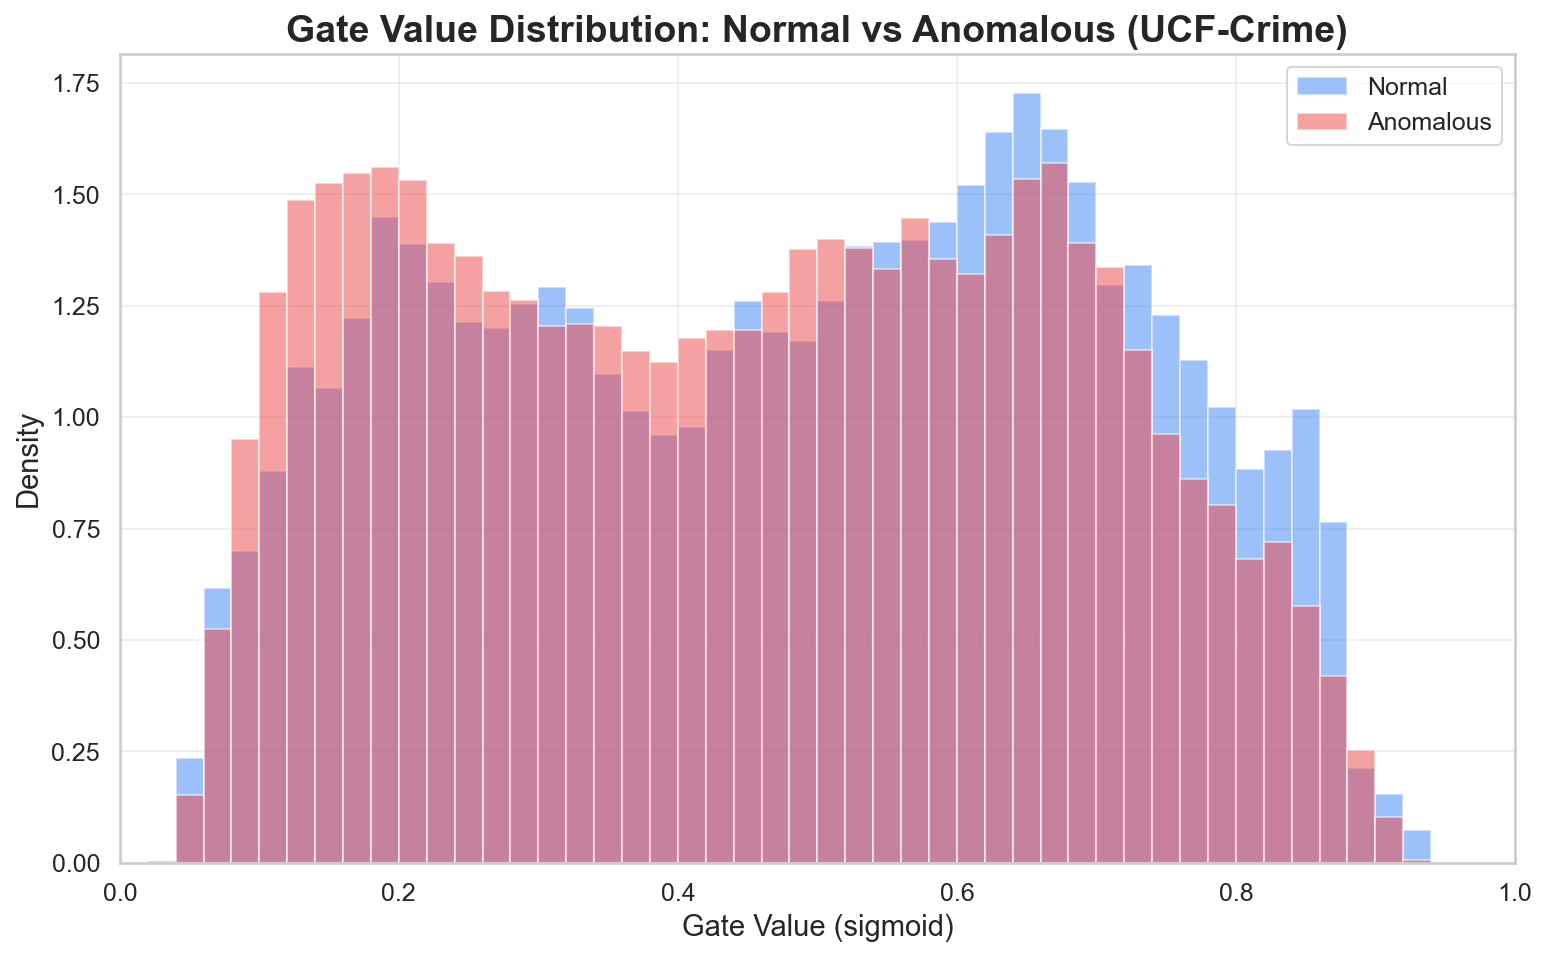
\includegraphics[width=\textwidth]{figures/fig_gate_histogram_ucf}
    \caption{UCF-Crime.}
  \end{subfigure}\hfill
  \begin{subfigure}[t]{0.48\textwidth}
    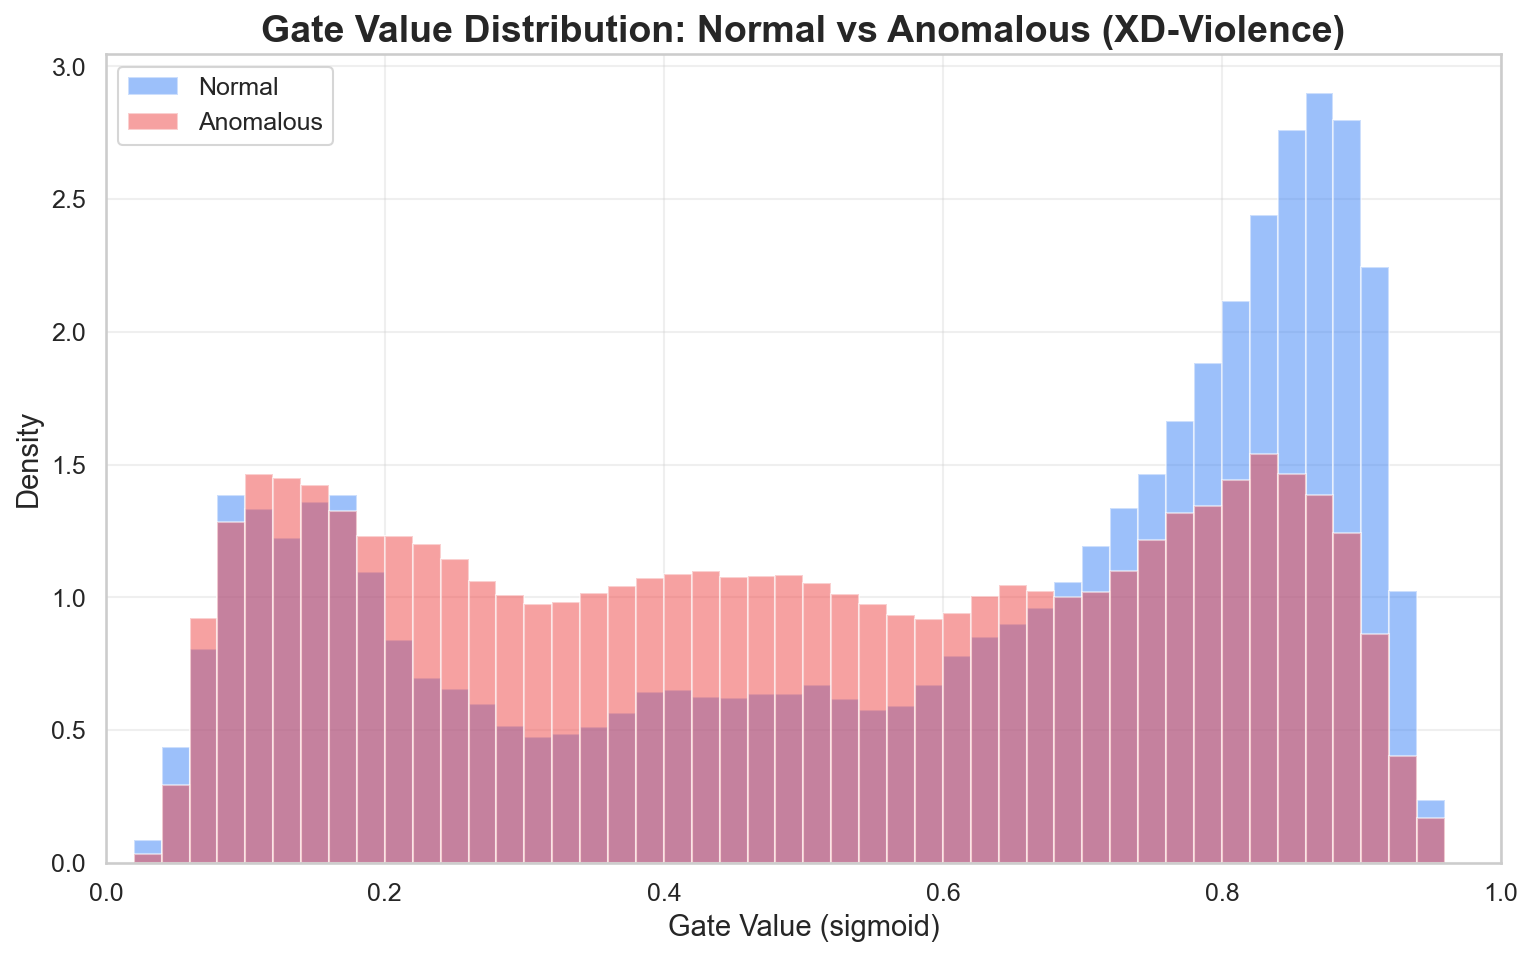
\includegraphics[width=\textwidth]{figures/fig_gate_histogram_xd}
    \caption{XD-Violence.}
  \end{subfigure}
  \caption{Distribution of learned gate activations for the gated-fusion
  models (seed 42), split by normal vs.\ anomalous test videos.
  Verification: regenerated from checkpoints that reproduce the tracked
  canonical metrics exactly under the official evaluation CLI; the UCF panel
  includes the corrected classification of the 150 in-annotation Normal test
  videos (PROVENANCE.md Class-V notes).}
  \label{fig:appf-gate-hist}
\end{figure}

\section{Per-Category Frame-Score Distributions}
\label{sec:appf-catscores}

Finally, Figure~\ref{fig:appf-catscores} shows the distribution of predicted
frame scores within anomalous test videos, grouped by category ---
information that the per-category AUC/AP tables of Appendix~\ref{app:b}
aggregate away. The spread within each category is wide: even
well-detected categories contain videos whose frames score across the full
range, which is the distributional face of the two failure regimes analyzed
in Chapter~\ref{ch:05} (saturated near-ties at the top of the range, and
short events whose frames are drowned in low-scoring context).

% Source: thesis/PROVENANCE.md §3 rows fig_category_scores_{ucf,xd} — Class V,
% regenerated 2026-07-05 from the validated s42 gated-fusion score dumps
% (frame-score distributions, abnormal videos only).
\begin{figure}[htbp]
  \centering
  \begin{subfigure}[t]{\textwidth}
    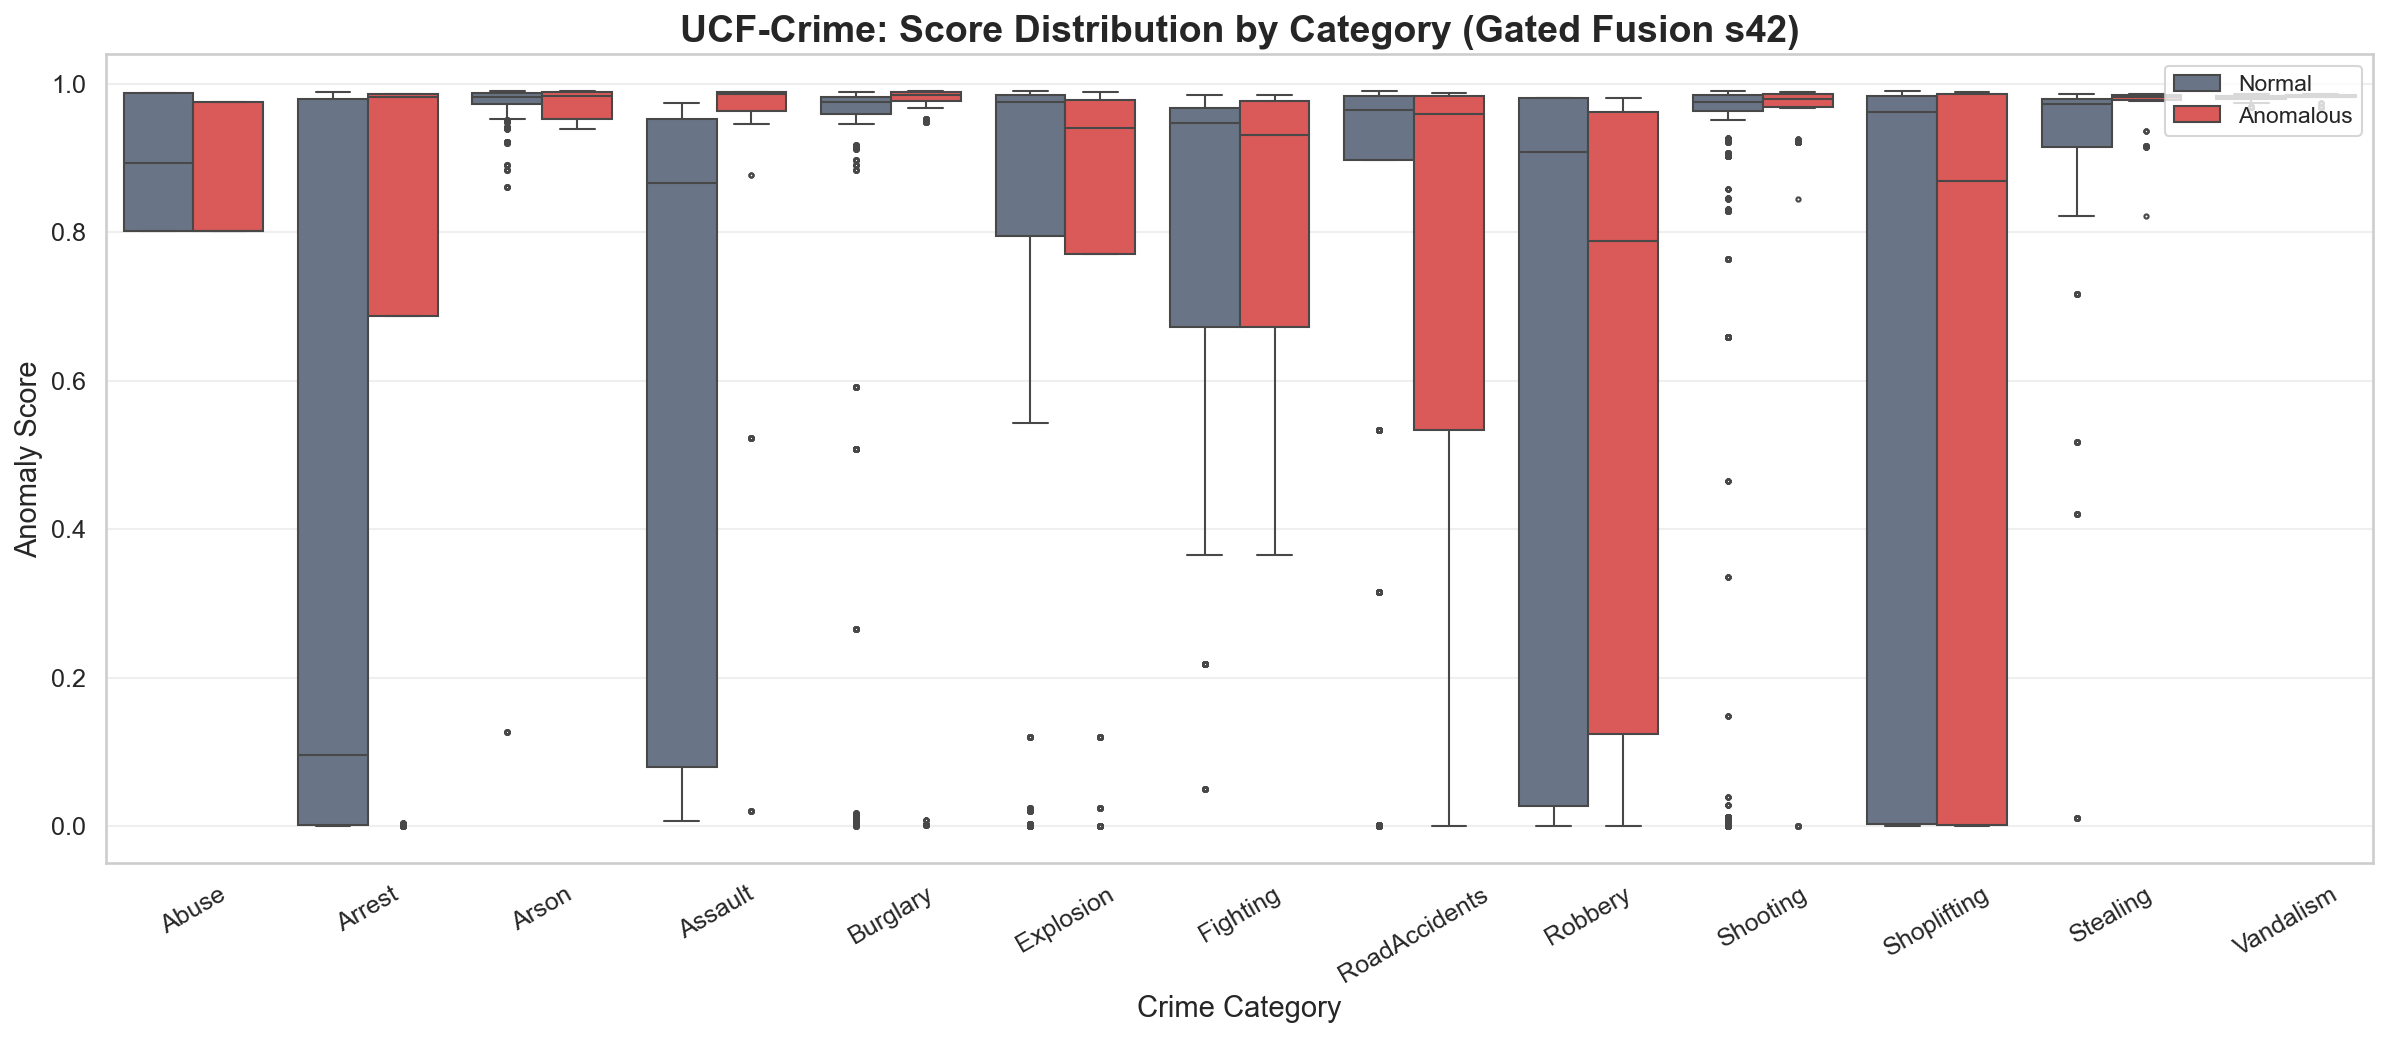
\includegraphics[width=\textwidth]{figures/fig_category_scores_ucf}
    \caption{UCF-Crime (13 anomaly categories).}
  \end{subfigure}\par\medskip
  \begin{subfigure}[t]{\textwidth}
    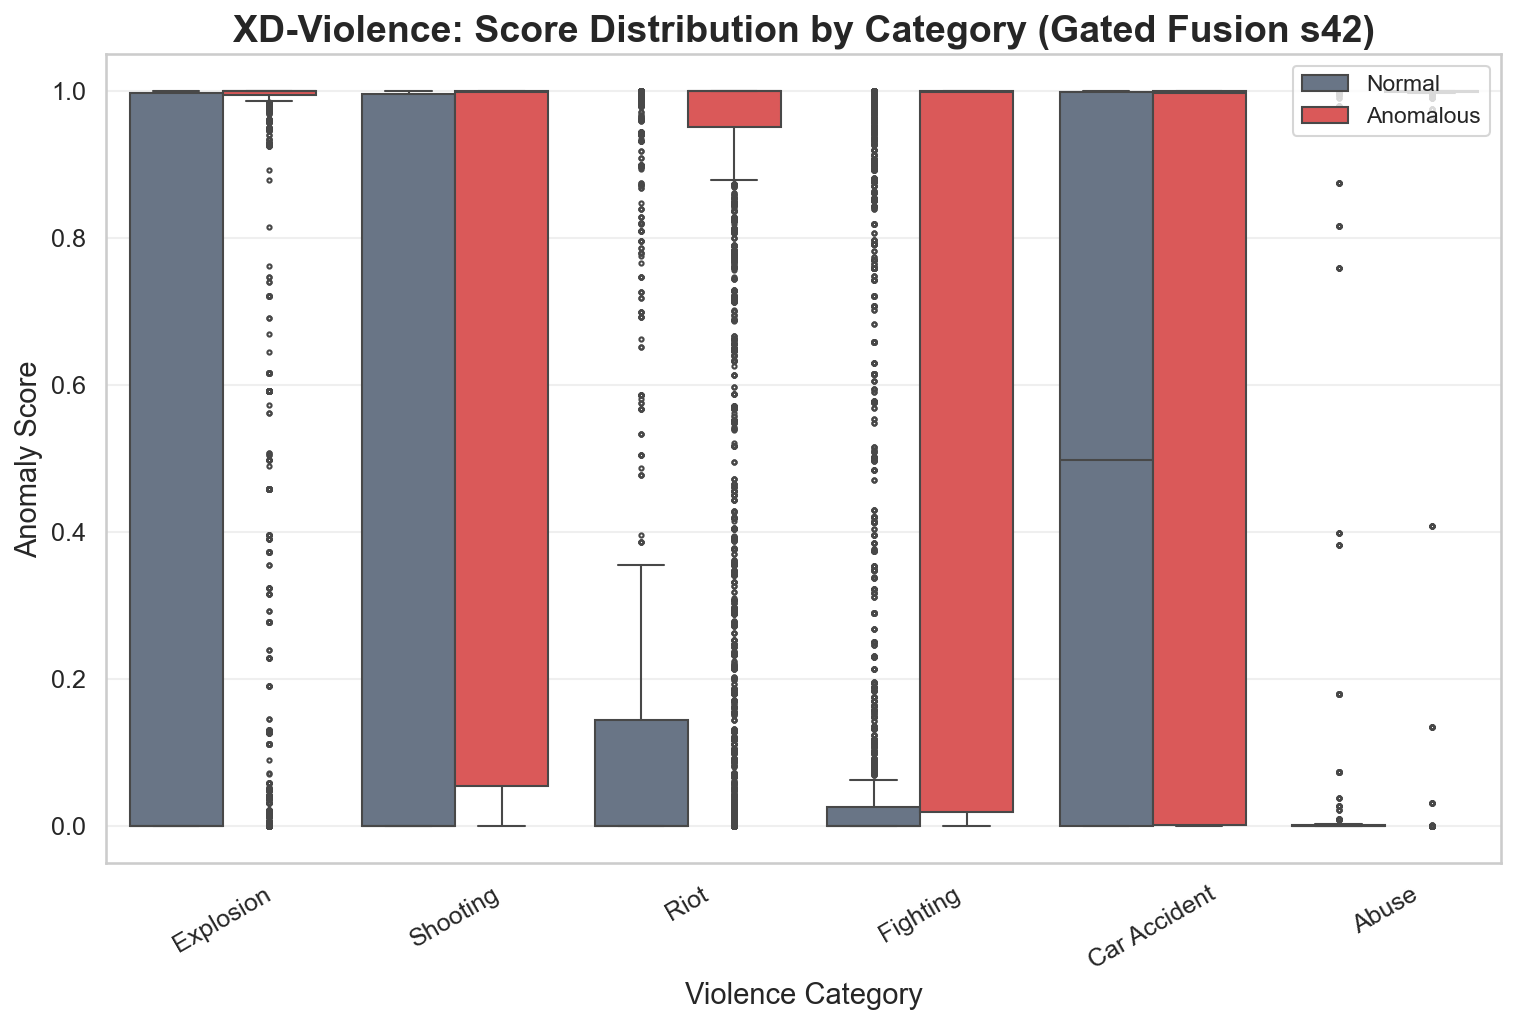
\includegraphics[width=\textwidth]{figures/fig_category_scores_xd}
    \caption{XD-Violence (6 anomaly categories).}
  \end{subfigure}
  \caption{Frame-score distributions by category for the gated-fusion models
  (seed 42), anomalous test videos only. Verification: regenerated from the
  same exactly-validated score dumps as
  Figure~\ref{fig:appf-temporal-ucf} (PROVENANCE.md Class-V notes).}
  \label{fig:appf-catscores}
\end{figure}
